\documentclass{article}

\title{Podstawy steganografii i stegoanalizy}
\author{Dominik Lau, Sebastian Kutny, Tomasz Lewandowski, Maciej Krzyżanowski}

\usepackage{blindtext}
\usepackage{amsmath}
\usepackage[utf8]{inputenc}
\usepackage[polish]{babel}
\usepackage[T1]{fontenc}
\usepackage{listings}
\usepackage{color}
\usepackage{amssymb}
\usepackage{esvect}
\usepackage{graphicx}
\usepackage{hyperref}
\usepackage{float}

\graphicspath{ {./obrazy/} }

\definecolor{dkgreen}{rgb}{0,0.6,0}
\definecolor{gray}{rgb}{0.5,0.5,0.5}
\definecolor{mauve}{rgb}{0.58,0,0.82}

\lstset{frame=tb,
  language=Python,
  aboveskip=3mm,
  belowskip=3mm,
  showstringspaces=false,
  columns=flexible,
  basicstyle={\small\ttfamily},
  numbers=none,
  numberstyle=\tiny\color{gray},
  keywordstyle=\color{blue},
  commentstyle=\color{dkgreen},
  stringstyle=\color{mauve},
  breaklines=true,
  breakatwhitespace=true,
  tabsize=3
}


\begin{document}

\maketitle
\section{Czym jest steganografia? Do czego służy?}
Steganografia polega na ukrywaniu informacji przez ukrywanie komunikacji w innej formie transmisji danych
np. w obrazkach,  plikach dźwiękowych, tekstowych.  Zastosowania steganografii
\begin{itemize}
	\item omijanie cenzury/szpiegostwo
	\item umieszczanie znaków wodnych
	\item ukryta wymiana danych
	\item dodawanie metadanych do plików (np. znaki sterujące)
	\item numery seryjne drukarek (za pomocą małych kropek)
	\item wprowadzanie opóźnień w pakietach sieciowych
	\item zastosowania w VoIP (steganofonia)
	\item zabezpieczanie banknotów (np. EURion constellation)
\end{itemize}
\begin{figure}
	\centering
	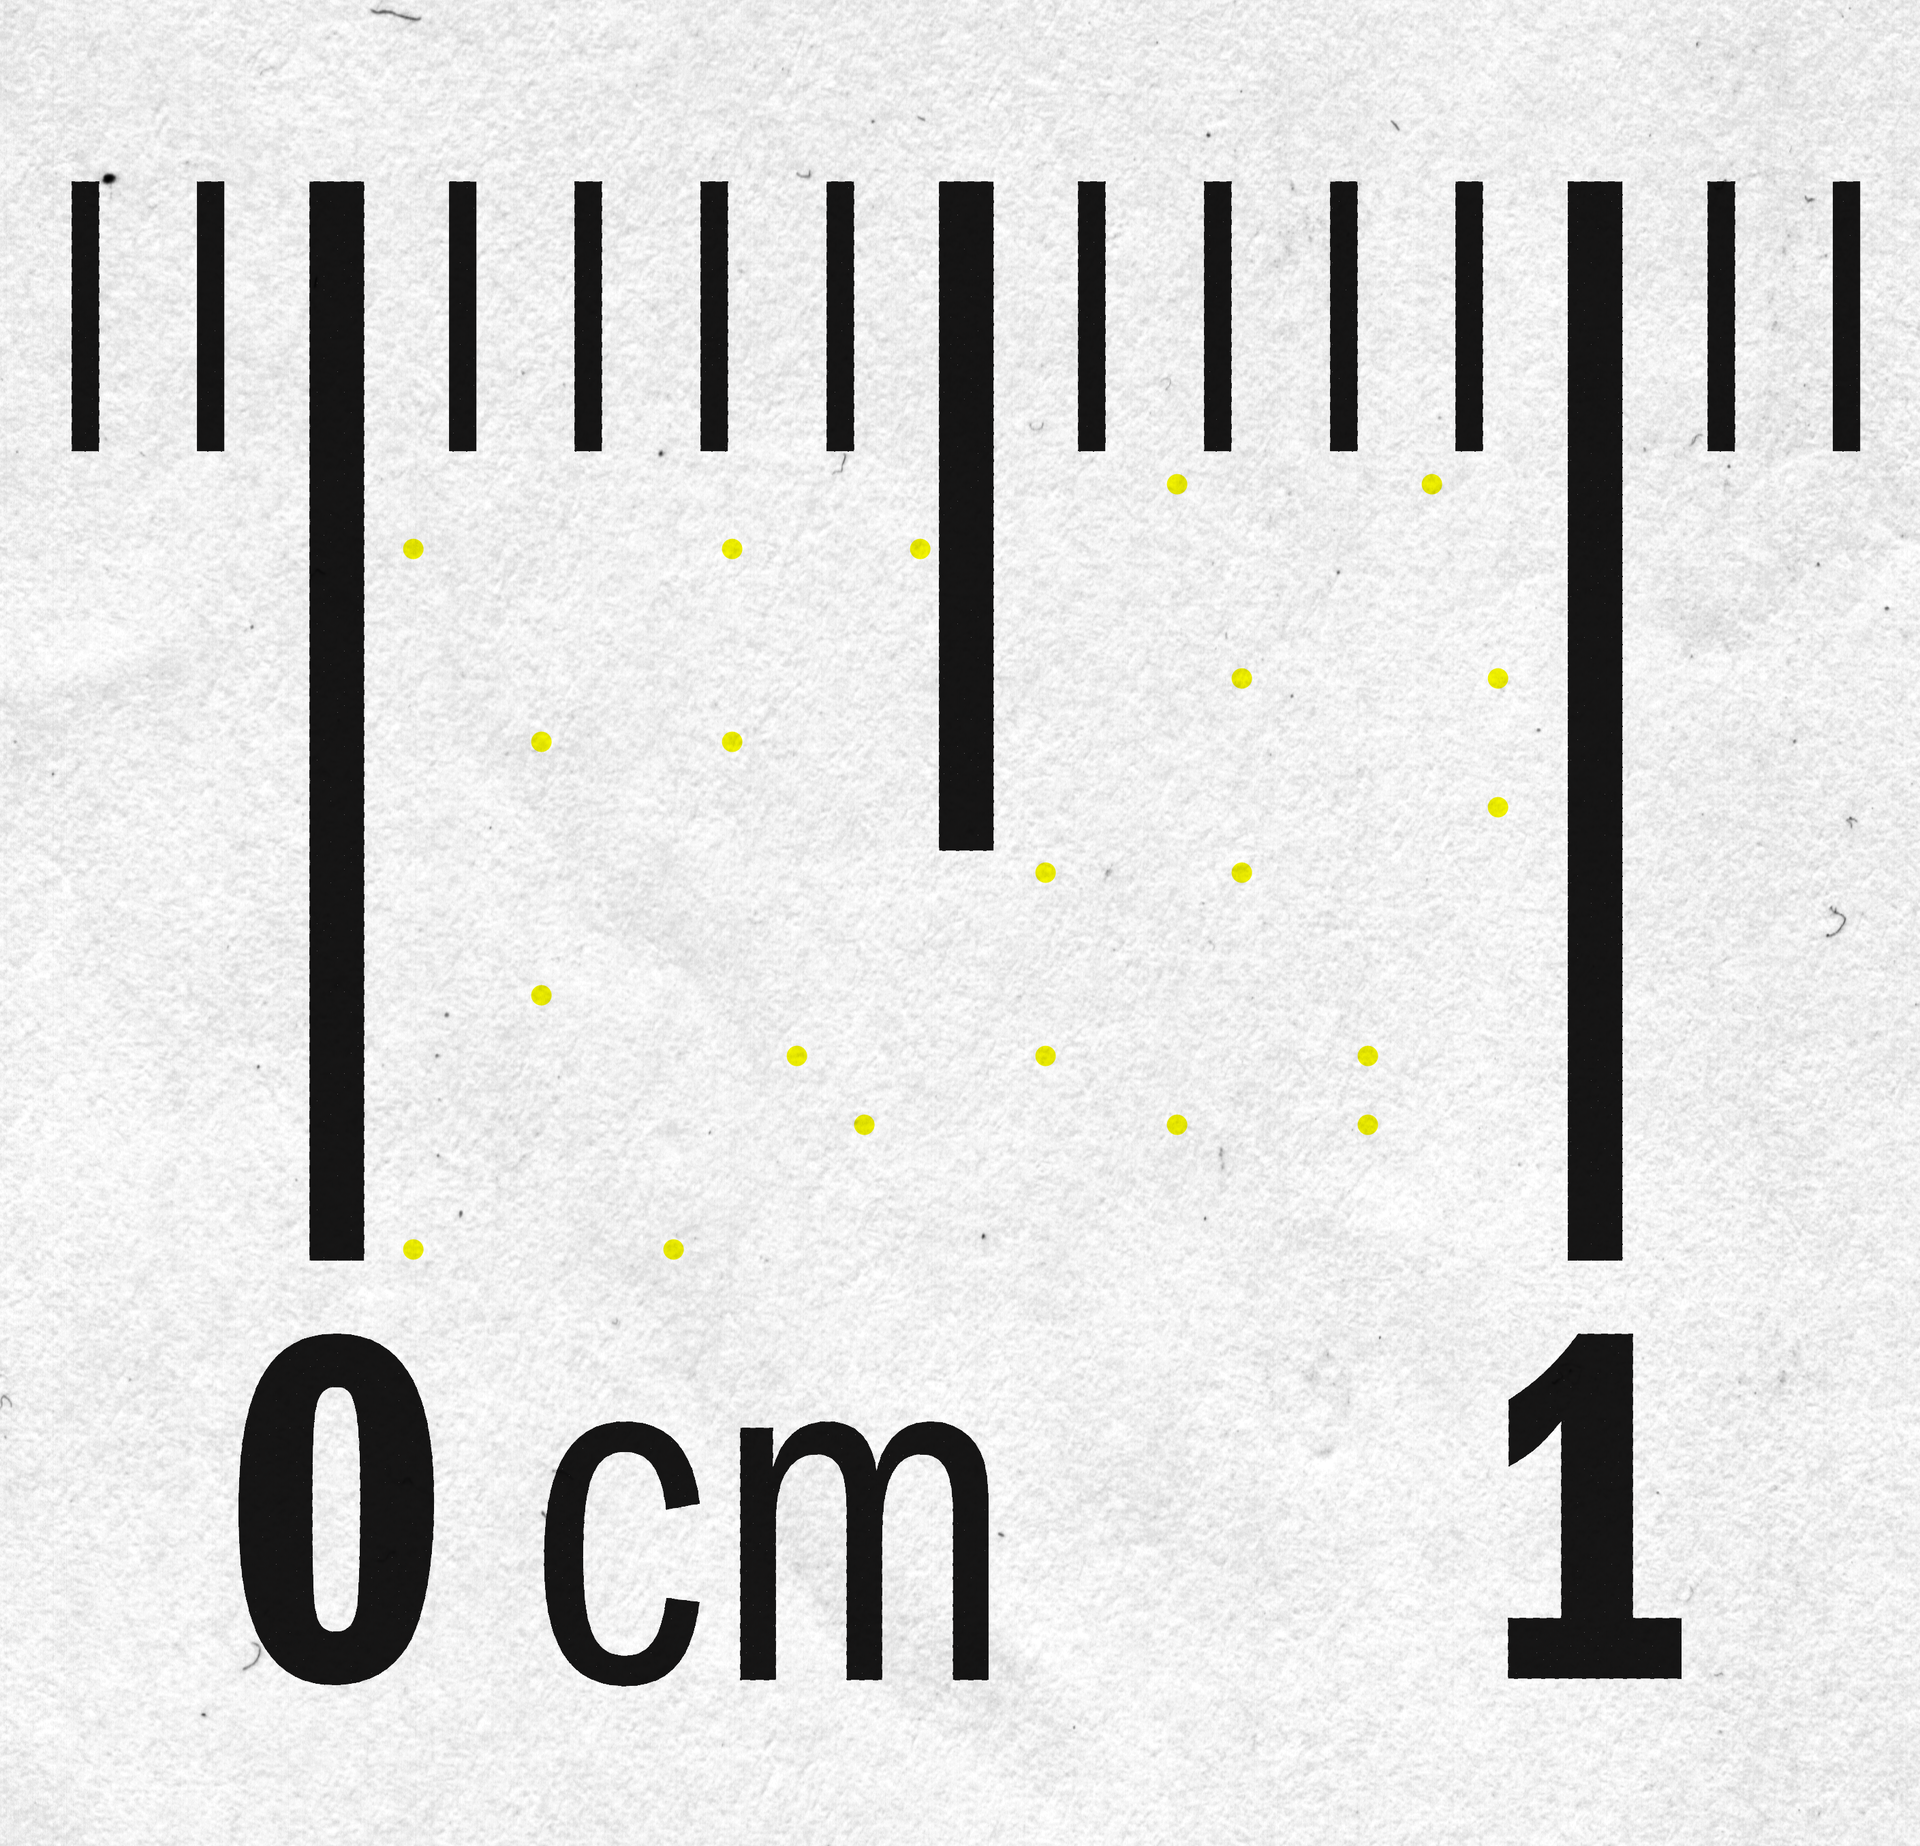
\includegraphics[width=5cm]{stego_drukarkowa}
	\caption{"kropki" zamieszczane przez drukarki}
\end{figure}
Steganografia może zatem realizować następujące funkcje bezpieczeństwa
\begin{itemize}
	\item poufność
	\item autentyczność
	\item niezaprzeczalność
	\item integralność
\end{itemize}
Porównanie kryptografii i steganografii
\begin{center}
\begin{tabular}{c | c  c }
& kryptografia & steganografia \\
\hline
cel & zapewnienie poufności & ukrycie komunikacji \\
obecność klucza & tak & opcjonalna \\
widoczność danych & nie & tak \\
modyfikacja struktury  \\
 przetwarzanych danych & nie & tak
\end{tabular}
\end{center}
\section{Podział steganografii}
Ze względu na sposób ukrywania danych
\begin{itemize}
	\item steganografia czysta - nie jest stosowany żaden klucz, tekst jawny ukrywamy w pliku, jest to metoda 	Security through obscurity (nie spełnia zasady Kerckhoffsa)
	\item steganografia z kluczem tajnym (symetrycznym) - przed komunikacją ustalany jest (np. algorytmem DH) klucz steganograficzny wykorzystywany potem w algorytmie, następnie ukrywamy tekst jawny w pliku
	\item steganografia z kluczem publicznym - w pliku ukrywamy szyfrogram zaszyfrowany kluczem publicznym
	odbiorcy
\end{itemize}
Ze względu na kontener
\begin{itemize}
	\item w plikach tekstowych
	\item w plikach audio
	\item w obrazach
	\item w ramkach różnych protokołów
	\item w plikach wykonawczych
	\item inne...
\end{itemize}
\section{Słowniczek}
\begin{itemize}
	\item stegosystem - połączenie metod i narzędzi służących do tworzenia ukrytego kanału do przekazywania informacji
	\item wiadomość (payload) - przesyłane dane
	\item kontener (carrier) - to wszelkie dane służące do ukrycia tajnej wiadomości
	\item stegokontener - dane i ukryta w nich tajna wiadomość
	\item kanał steganograficzny (stegochannel) - kanał transmisji stegokontenera
	\item klucz (stegokey) - tajny klucz potrzebny do ukrycia stegokontenera
\end{itemize}
\begin{figure}
	\centering
	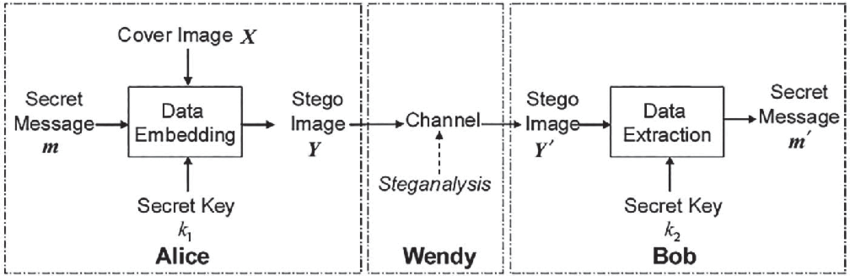
\includegraphics[width=8cm]{model_steganografii}
	\caption{model steganografii}
\end{figure}
\section{Historia steganografii}
\section{Algorytmy i przykłady}
W tej sekcji prezentujemy wybrane algorytmy steganografii na obrazach oraz przykładowe zastosowania
\subsection{Modyfikacja LSB}
\textbf{Zakodowanie} \\
Jest to klasyczny algorytm steganografii, którego główną wadą jest łatwość w wykryciu/zniszczeniu wiadomości
(np. przez wyzerowanie najmłodszych bitów). Przed niechcianym odczytem wiadomości możemy zapobiec 
poprzez zastosowanie kryptografii. Zasada działania algorytmu jest prosta:
\begin{enumerate}
	\item wybierz, w którym kanale zapisać bity wiadomości (r,g,b, a, może obraz czarnobiały?)
	\item zastąp stare wartości najmłodszych bitów określonego kanału obrazu kolejnymi bitami wiadomości
\end{enumerate}
Analogiczna metoda jest możliwa na plikach dźwiękowych, tylko tam zmieniamy LSB próbek. \\\\
\textbf{Detekcja} \\
Prosta metoda wykrycia, czy obraz zawiera zakodowaną wiadomość
\begin{enumerate}
	\item dzielimy piksele na bloki
	\item dla każdego bloku liczymy wartość średnią LSB
\end{enumerate}
Jeżeli w obrazie ukryto \textbf{zaszyfrowaną} wiadomość, to niektóre regiony bloków
powinny mieć średnią $\approx 0.5$

\subsection{Gamma trick*}
\subsection{Ukrywanie obrazów w spektrogramach}

\subsection{Eurion}
\begin{figure}[H]
	\centering
	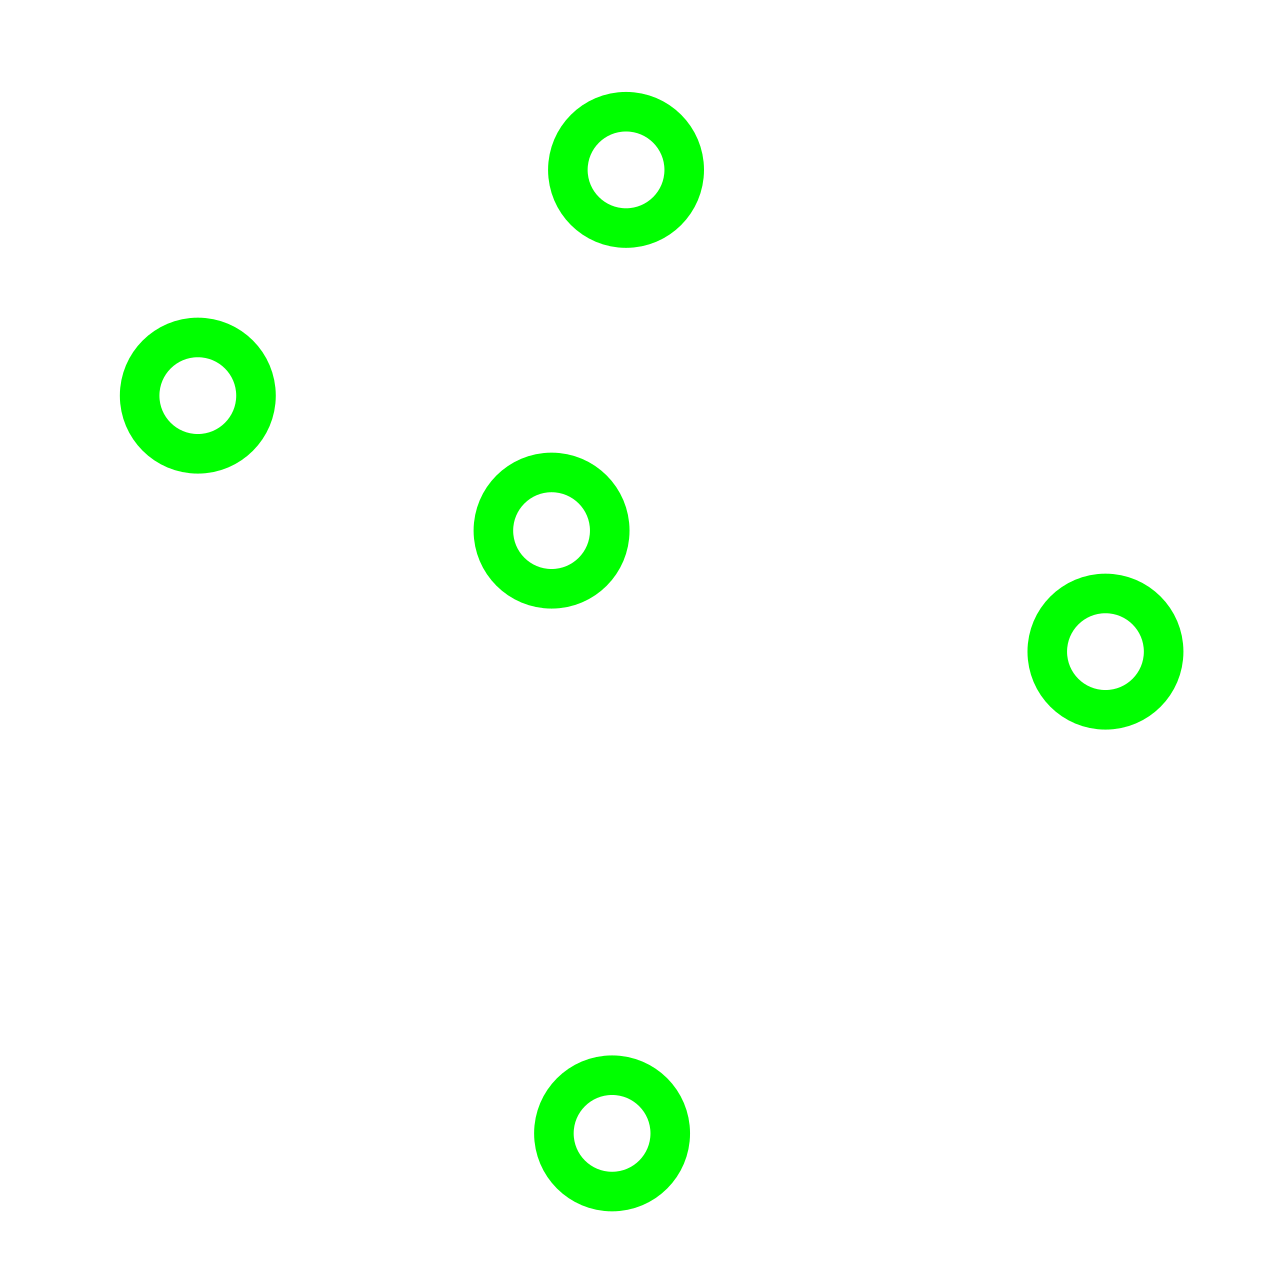
\includegraphics[width=5cm]{eurion}
	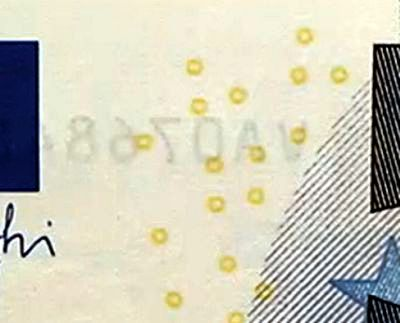
\includegraphics[width=5cm]{euro}
	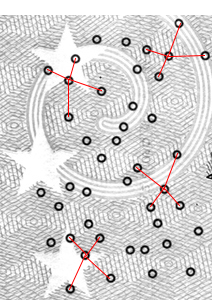
\includegraphics[width=5cm]{close}
	\caption{EURion, przykładowy układ na banknocie euro, dollarze}
\end{figure}
EURion jak i inne podobne zabiegi stanowią metodę przeciwdziałania fałszerstwom. Na banknotach umieszczane
są zbiory kropek o różnych średnicach i względnych pozycjach (te parametry są sekretem). Kropki te tworzą
fingerprint, który jest wykrywany przez oprogramowanie do skanowania (za pomocą metod detekcji wzorca) i
wszelkie próby kopiowania banknotów są blokowane.  
\section{Narzędzia steganograficzne}
\section{Źródła}
\begin{itemize}
	\item \url{https://pl.wikipedia.org/wiki/Steganografia_drukarkowa}
	\item \url{https://royalprice.ru/pl/setting/steganografiya-i-stegoanaliz-obzor-sushchestvuyushchih-programm-i-algoritmov/}
	\item \url{https://www.researchgate.net/figure/The-model-of-steganography-and-steganalysis_fig1_333772050}
	\item \url{http://datagenetics.com/blog/september12015/index.html}
\end{itemize}

\end{document}
